\begin{exercise}
\begin{figure}[H]
\centering
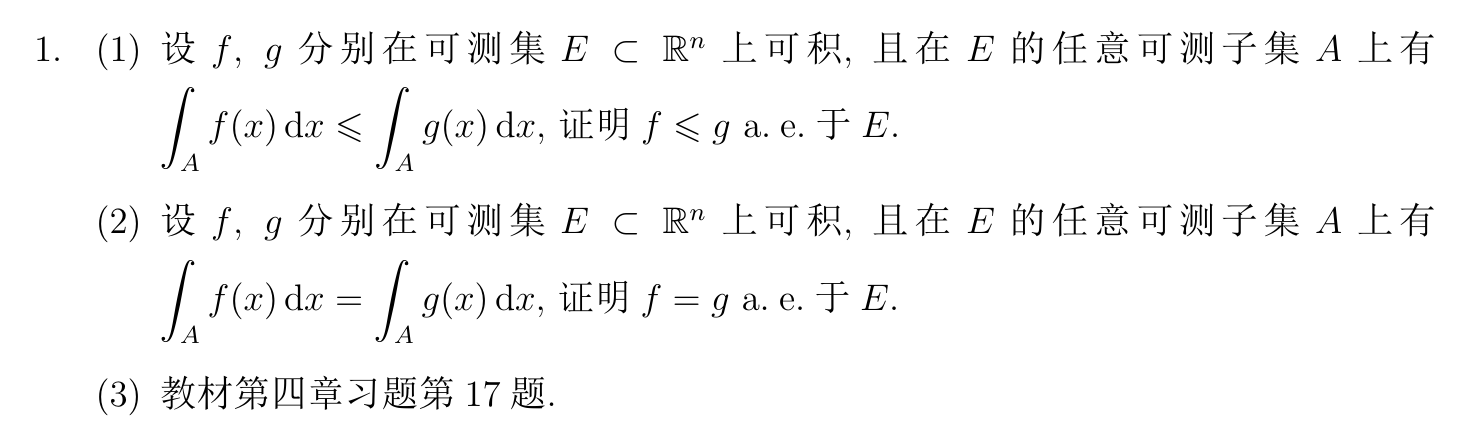
\includegraphics[width=\textwidth]{hw12-2025052108.png}
% \caption{}
\label{}
\end{figure}
\begin{figure}[H]
\centering
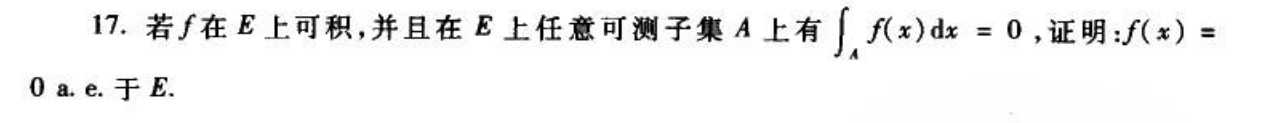
\includegraphics[width=\textwidth]{1-hw12-2025052108.png}
% \caption{}
\label{}
\end{figure}
\end{exercise}
(1)
If $f>g$ on $A$, $mA>0$, then
\[
\int_{A}^{} f \, \mathrm{d}x >\int_{A}^{} g \, \mathrm{d}x
\]
Contradiction!

(2)
Apply (1). $f\geq g$ a.e. on $E$, $f\leq g$ a.e. on $E$; thus $f=g$ a.e. on $E$.

(3)
Put $g\equiv0$ in (2), then $f(x)=0$ a.e. on $E$.

\begin{exercise}
\begin{figure}[H]
\centering
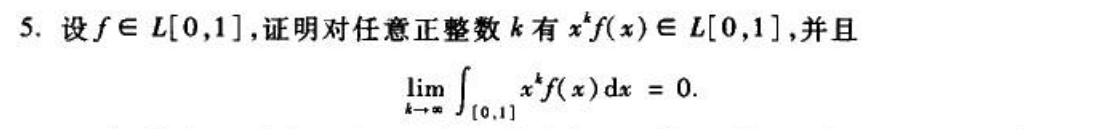
\includegraphics[width=\textwidth]{2-hw12-2025052108.png}
% \caption{}
\label{}
\end{figure}
\end{exercise}
$f\in L[0,1]$ iff $f^{+},f^{-}\in L[0,1]$. As $(x^{k}f(x))^{+}=x^{k}f^{+}(x),(x^{k}f(x))^{-}=x^{k}f^{-}(x)$,
\[
\int_{[0,1]}^{} \lvert x^{k}f^{+}(x)  \rvert \, \mathrm{d}x \leq \int_{[0,1]}^{} \lvert f^{+}(x) \rvert  \, \mathrm{d}x <\infty
\]
\[
\int_{[0,1]}^{} \lvert x^{k}f^{-}(x) \rvert  \, \mathrm{d}x \leq \int_{[0,1]}^{} \lvert f^{-}(x) \rvert  \, \mathrm{d}x <\infty
\]
$x^{k}f^{+}, x^{k}f^{-}\in L[0,1]$, then $x^{k}f\in L[0,1]$.
\[
\lim_{ k \to \infty } x^{k}f(x)=\begin{cases}
0 & x\in[0,1) \\
f(1) & x=1
\end{cases}
\]
By DCT,
\[
\lim_{ k \to \infty } \int_{[0,1]}^{} x^{k}f(x) \, \mathrm{d}x = \int_{[0,1]}^{} \lim_{ k \to \infty } x^{k}f(x) \, \mathrm{d}x =\int_{\{ 1 \}}^{} f(1) \, \mathrm{d}x =0
\]
\begin{exercise}
\begin{figure}[H]
\centering
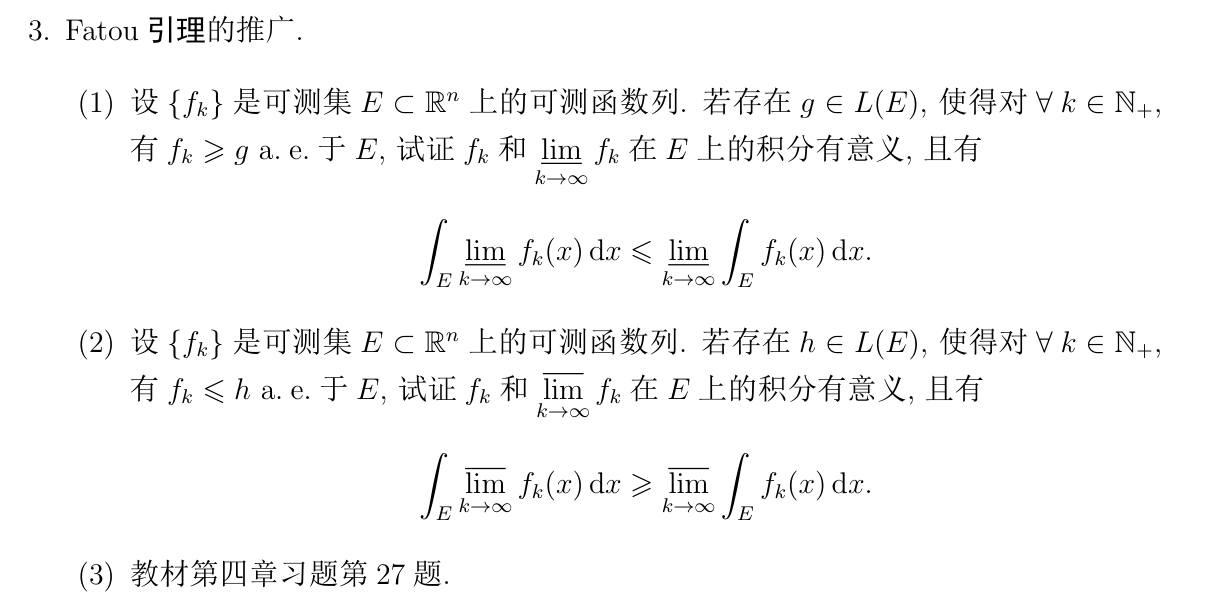
\includegraphics[width=\textwidth]{3-hw12-2025052108.png}
% \caption{}
\label{}
\end{figure}
\begin{figure}[H]
\centering
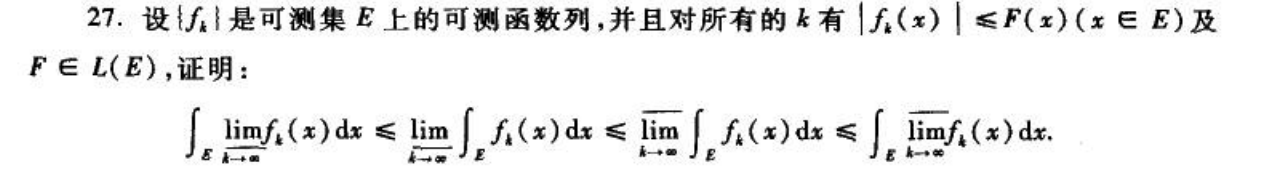
\includegraphics[width=\textwidth]{5-hw12-2025052108.png}
% \caption{}
\label{}
\end{figure}\label{c2dff9}
\end{exercise}

(1) 对任意 $E$ 上可测的 $f\geq g$, $f^{-}=\min\{ 0,f \}\geq \min\{ 0,g \}=g^{-}$, 由于 $g\in L(E)$,则 $\int_{E}^{} g^{-}>-\infty$,故 $\int_{E}f^{-}\geq \int_{E}g^{-}>-\infty$,故 $\int_{E}f^{+}$ 和 $\int_{E}f^{-}$ 不同时为 $\infty$,故 $\int _Ef$ 有定义. 由于 $f_k\geq g,\varliminf_{ k \to \infty }f_k\geq g$,故 $\int_{E}f_k$, $\int_{E}\varliminf_{ k \to \infty }f_k$ 有定义. 由于 $\varliminf_{ k \to \infty }f_k\leq f_k$ 于 $E$, $k$ 任意,故 $\int_{E}\varliminf_{ k \to \infty }f_k\leq \int_{E}f_k$,对右边关于 $k$ 取下极限,得到 $\int _E\varliminf_{ k \to \infty }f_k\leq \varliminf_{ k \to \infty }\int_{E}f_k$.

(2) 考虑 $-f_k$, $-f_k\geq-h$, $h\in L (E)\Rightarrow -h\in L(E)$. 于是 $\int_{E}(-f_k)$, $\int_{E}\varliminf_{ k \to \infty }(-f_k)$ 有定义,其中 $(-f_k)^{-}=\min\{ 0,-f_k \}=-\max\{ 0, f_k \}=-f_k^{+}, (-f_k)^{+}=-f_k^{-}$, $\varliminf_{ k \to \infty }(-f_k)=\lim_{ n \to \infty }\inf_{k\geq n}(-f_k)=\lim_{ n \to \infty }(-\sup_{k\geq n}f_k)=-\varlimsup_{ k \to \infty }f_k$. 因此 $f_k^{+},f_k^{-}$ 不同时为 $\infty$, $(\varlimsup_{ k \to \infty }f_k)^{+},(\varlimsup_{ k \to \infty }f_k)^{-}$ 不同时为 $\infty$, 故 $\int_{E}f_k,\int_{E}\varlimsup_{ k \to \infty }f_k$ 有意义. 由 (1) 可知 $\int_{E}\varliminf_{ k \to \infty }(-f_k)\leq \varlimsup_{ k \to \infty } \int _E(-f_k)$. 故
$\int_{E}\varlimsup_{ k \to \infty }f_k\geq \varlimsup_{k\to \infty}\int_{E}f_k$.

(3) 对于数列 $\left\{  \int_{E}^{} f_k(x) \, \mathrm{d}x  \right\}_{k\geq1}$ ,显然有 $\varliminf_{ k \to \infty }\int_{E}f_k\leq \varlimsup_{ k \to \infty }\int_{E}f_k$,根据 $-F\leq f_k\leq F$, $F\in L (E),-F\in L(E)$ ,结合 (1)(2) 可知
\[
\int_{E}^{} \varliminf_{ k \to \infty } f_k(x) \, \mathrm{d}x \leq \varliminf_{ k \to \infty } \int_{E}^{} f_k(x) \, \mathrm{d}x \leq \varlimsup_{ k \to \infty } \int_{E}^{} f_k(x) \, \mathrm{d}x \leq \int_{E}^{} \varlimsup_{ k \to \infty } f_k(x) \, \mathrm{d}x
\]
\begin{exercise}
\begin{figure}[H]
\centering
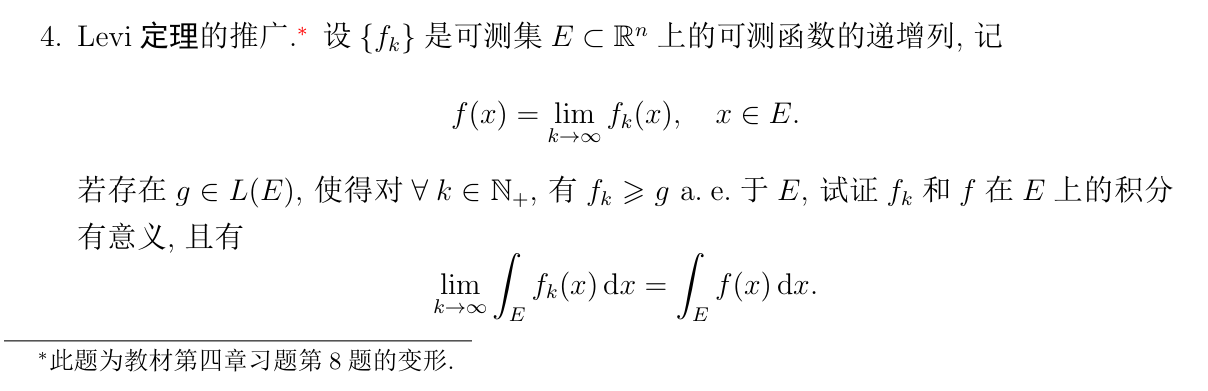
\includegraphics[width=\textwidth]{6-hw12-2025052108.png}
% \caption{}
\label{}
\end{figure}
\end{exercise}
类似 \cref{c2dff9} 中的讨论,可知 $f_k,f$ 在 $E$ 上积分有意义,对于非负递增可测函数列 $\{ f_k-g \}_{k\geq1}$,我们有 Levi 定理可知 $\lim_{ k \to \infty }\int_{E}^{} (f_k-g)=\int_{E}(f-g)$. 由积分的线性性可知
\[
\lim_{ k \to \infty } \int_{E}^{} f_k(x) \, \mathrm{d}x =\int_{E}^{} f(x) \, \mathrm{d}x
\]
\begin{exercise}
\begin{figure}[H]
\centering
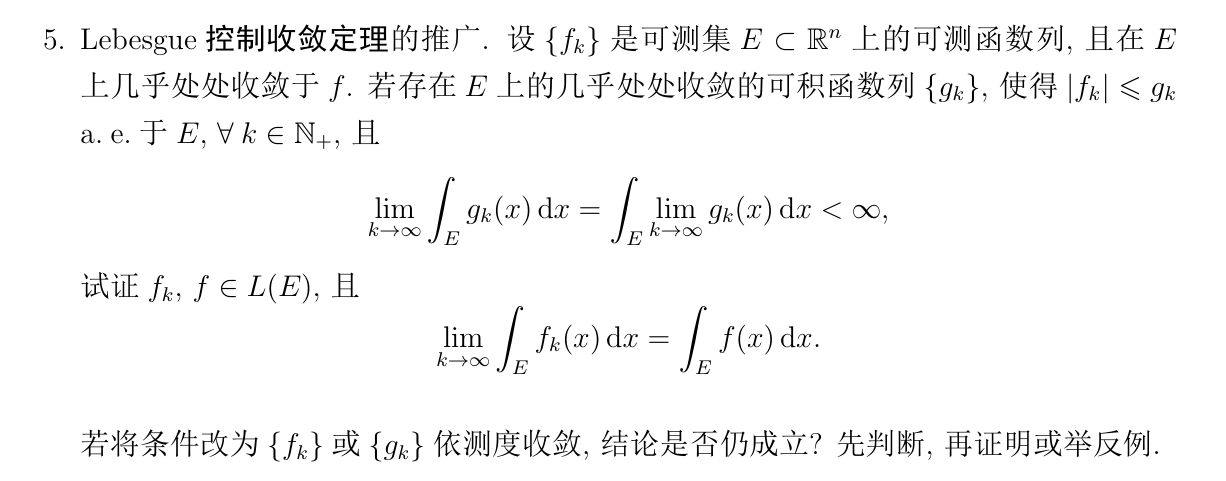
\includegraphics[width=\textwidth]{7-hw12-2025052108.png}
% \caption{}
\label{}
\end{figure}\label{1fa9d0}
\end{exercise}

由比值判别法,$f_k$ 可积. 记 $g_k$ 几乎处处收敛于 $g$,则 $\int_{E}g=\int_{E}\varliminf_{ k \to \infty }g_k\leq \varliminf_{ k \to \infty }\int_{E}g_k$, 故 $g\in L(E)$. 令 $k\to \infty$,则 $\lvert f \rvert\leq g$, 由比值判别法,$g\in L(E)$. 考虑非负可测函数列 $\{ g_k-f_k \}_{k\geq1}$,它几乎处处收敛于 $g-f$. 利用 Fatou 引理,$\int_{E}(g-f)\leq \varliminf_{ k \to \infty }\int_{E}(g_k-f_k)$, 于是
\[
\int_{E}g-\int_{E}f=\int_{E}(g-f)\leq \varliminf_{ k \to \infty } \int_{E}g_k-\varlimsup_{ k \to \infty } \int_{E}f_k=\int_{E}g-\varlimsup_{ k \to \infty } \int_{E}f_k
\]
于是 $\varlimsup_{ k \to \infty }\int_{E}f_k\leq \int_{E}f$. 再考虑非负可测函数列 $\{ f_k+g_k \}$ 得到 $\int_{E}f\leq \varliminf_{ k \to \infty }\int_{E}f_k$. 因此 $\lim_{ k \to \infty }\int _Ef_k=\int_{E}f$.

若 $f_k\overset{ m }{ \to }f$,对于任意子列 $\{ f_{k_{n}} \}$,存在子列 $\{ f_{k_{n_{m}}} \}\to f$ a.e. 于 $E$. 从而 $f\in L(E)$, $\lim_{ m \to \infty }\int_{E}f_{k_{n_m}}=\int_{E}f$. 对于数列 $\left\{  \int_{E}f_{k}  \right\}$,它的任意子列 $\left\{  \int_{E} f_{k_{n}} \right\}$ 都含有子列 $\left\{  \int_{E}f_{k_{n_{m}}}  \right\}\to \int_{E}f$,不妨考虑 $\left\{  \int_{E}f_k  \right\}$ 的上下极限序列,它们都含有子列收敛于 $\int_{E}f$,故 $\lim_{ k \to \infty }\int _Ef_k=\int_{E}f$.

若 $g_k\overset{ m }{ \to }g$, 同样考虑 $\{ f_k \}$ 的任意子列,再选取子列 $k_{n}$ 使得 $g_{k_n}\to g$ a.e. 于 $E$, 重复上述论述即可得证.

\begin{exercise}
\begin{figure}[H]
\centering
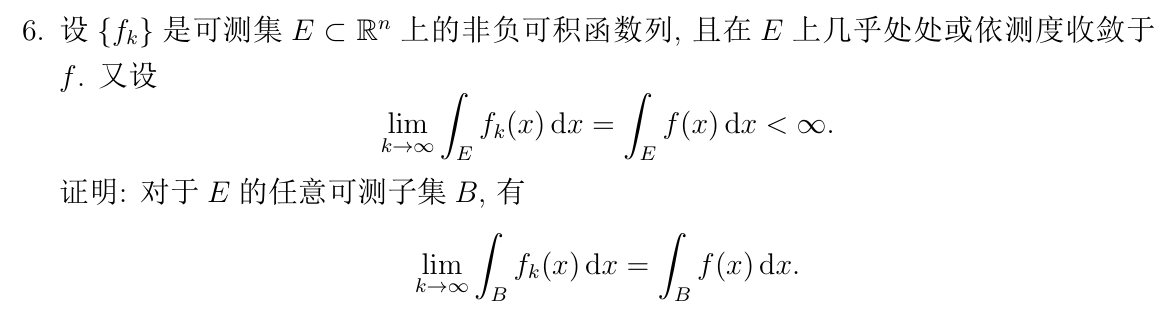
\includegraphics[width=\textwidth]{8-hw12-2025052108.png}
% \caption{}
\label{}
\end{figure}
\end{exercise}
令 $g_k=f_k\chi_{B}$,于是 $\lvert g_k \rvert\leq f_k$,利用 \cref{1fa9d0} 立得 $\lim_{ k \to \infty }\int_{E}^{} g_k \, \mathrm{d}x=\int_{E}^{} g(x) \, \mathrm{d}x$, 也就是 $\lim_{ k \to \infty }\int_{B}^{} f_k(x) \, \mathrm{d}x=\int_{B}^{} f(x) \, \mathrm{d}x$.

\begin{exercise}
\begin{figure}[H]
\centering
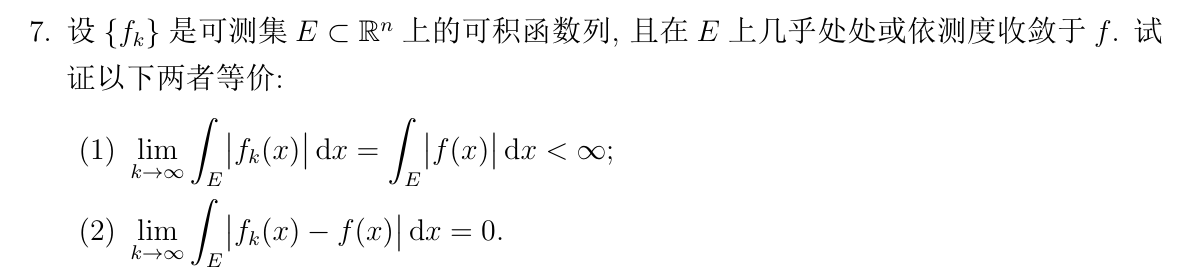
\includegraphics[width=\textwidth]{9-hw12-2025052108.png}
% \caption{}
\label{}
\end{figure}
\end{exercise}
若 $\lim_{ k \to \infty }\int _E\lvert f_k-f \rvert=0$,则 $\int_{E}\lvert \lvert f_k \rvert-\lvert f \rvert \rvert\leq \int_{E}\lvert f_k-f \rvert\to0$. 若 $\int_{E}\lvert f_k \rvert\to \int_{E}\lvert f \rvert<\infty$, 注意到 $\lvert f_k-f \rvert\leq \lvert f_k \rvert+\lvert f \rvert$,由 DCT
\[
\lim_{ k \to \infty } \int_{E}\lvert f_k-f \rvert =\int_{E}\lim_{ k \to \infty } \lvert f_k-f \rvert =\int_{E}0=0
\]
\begin{exercise}
\begin{figure}[H]
\centering
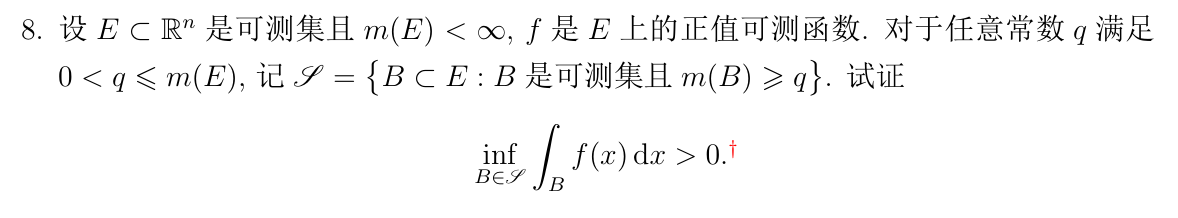
\includegraphics[width=\textwidth]{10-hw12-2025052108.png}
% \caption{}
\label{}
\end{figure}
\end{exercise}
考虑反证,假设 $\inf_{B\in \mathscr{S}}\int_{B}f=0$, 则存在 $\{ B_k \}\subset \mathscr{S}$ 使得

\begin{enumerate}
	\item $B_k\subset E$
	\item $m(B_k)>q$
	\item $\int_{B_k}f\to0$
\end{enumerate}

记 $F_j=E\left( f\leq \frac{1}{j} \right)$. 于是 $\lim_{ j \to \infty }m(F_j)=m\left( \bigcap_{j=1}^{\infty}F_j \right)=m(E(f=0))=0$, 从而存在 $J$ 使得 $m(F_J)<\frac{q}{2}$,故
\[
\int_{B_k}f=\int_{B_k\cap F_{J}}f+\int_{B_k\cap F_{J}^{c}}f\geq \int_{B_k\cap F_{J}^{c}}f\geq \frac{1}{J}m(B_k\cap F_{J}^{c})
\]
令 $k\to \infty$,就有 $m(B_k\cap F_{J}^{c})\to0$, 存在 $K$ 使得 $m(B_{K}\cap F_{J}^{c})<\frac{q}{2}$,故
\[
m(B_{K})=m(B_{K}\cap F_{J})+m(B_{K}\cap F_{J}^{c})\leq m(B_{K})+m(B_{K}\cap F_{J}^{c})<\frac{q}{2}+\frac{q}{2}=q
\]
矛盾!

\begin{exercise}
\begin{figure}[H]
\centering
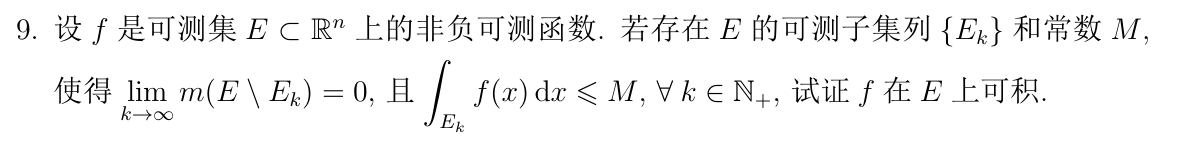
\includegraphics[width=\textwidth]{11-hw12-2025052108.png}
% \caption{}
\label{}
\end{figure}
\end{exercise}
$f_k\coloneqq f\cdot\chi_{E_k}$, then
\[
E(f_k \not\to f)=E(f(\chi_{E_k}-1)\not\to0)\subset E(\chi_{E\setminus E_k}\not\to0)=\bigcap_{k=1}^{\infty} (E\setminus E_k)
\]
Then $m(E(f_k\not\to f))\leq m\left( \bigcap_{k=1}^{\infty}(E\setminus E_k) \right)\leq m(E\setminus E_k),\forall k$. Let $k\to \infty$, then
\[
m(E(f_k\not\to f))=0
\]
Thus $f_k\to f$ a.e. on $E$. As $\int_{E}^{} f_k(x) \, \mathrm{d}x\leq M$, by BCT,
\[
\int_{E}f=\lim_{ k \to \infty } \int_{E}f_k\leq M
\]
Since $f$ is nonnegative measurable, $f$ is integrable.
